\documentclass{article}
\usepackage{../lambdatex} %disponibile all'indirizzo http://lambdamath.altervista.it/esercizi/lambdatex.sty
\usepackage{tasks}
\usepackage{exsheets}
\newcommand{\se}{\text{ se }}
\renewcommand{\phi}{\varphi}
\everymath{\displaystyle}

\title{Università degli Studi di Trento - Dipartimento di Matematica\\
CdL in Matematica – a.a. 2022–2023\\ Note esercitazione}
\author{Esercitatore: Simone Verzellesi\thanks{Trascrizione a cura di Davide Borra}}
\date{12 Dicembre 2022}
\begin{document}
\maketitle
\lhead{Note esercitazione}
\chead{Università degli Studi di Trento - Dipartimento di Matematica\\
CdL in Matematica – a.a. 2022–2023}
\rhead{12/12/2022}
\setlength{\headheight}{30pt}
% \begin{question}
%     pippo
%\end{question}
\begin{enumerate}[label=\textbf{Esercizio 12.\arabic*.},itemindent=*]
%%%%%%%%%%%%%%%%%%%%%%%%%%%%%%%%%%%%%%%%%%%%%%%%%%%%%
\item Siano $f(s)=\frac{e^{-|s|}-1}{s(s+1)}$ e $F(x)=\int_0^xf(s)ds$
\begin{tasks}
    \task Studiare $f(s)$
    \task Determinare $\dom F$
    \task Determinare $G_F$
\end{tasks}
\item[\textit{\large Soluzione~}]~
\begin{enumerate}
    \item Studiare $f(s)$
    \begin{itemize}
        \item $\dom f=\R\setminus\{0,1\}$
        \item Segno di $f$:
        \[e^{-|s|}-1\leq 0~~\forall s\in \R\]
        \[s(s+1)>0~~\Harr~~s<1\lor s>0\]
        Quindi
        \[f(s)>0 \se -1<s<0\]
        \[f(s)<0 \se s<0 \lor s>-1\]
        \item Limiti
        \[\lim_{s\to-\infty}f(s)=0^-\]
        \[\lim_{s\to1^-}f(s)=\left[ \frac{1-\frac{1}{e}}{0^-} \right]=-\infty\]
        \[\lim_{s\to1^+}f(s)=\left[ \frac{1-\frac{1}{e}}{0^+} \right]=+\infty\]
        \[\lim_{s\to0^-}f(s)=\lim_{s\to 0}\frac{e^s-1}{s(s+1)}\stackrel{LN}{=}1\]
        \[\lim_{s\to0^+}f(s)=\lim_{s\to 0}\frac{e^{-s}-1}{s(s+1)}\stackrel{LN}{=}-1\]
        \item Derivata di $f$
        \[f'(s)=\begin{cases}
            \frac{-e^{-s}(s^2+3s+1)+(2s+1)}{s^2(s+1)^2}&\se s>0\\
            \frac{e^{s}(s^2-s-1)+(2s+1)}{s^2(s+1)^2}&\se s<0\\
        \end{cases}\]
        \begin{itemize}
            \item se $s>0$
            \[f'(s)<0~~\Harr~~-e^{-s}(s^2+3s+1)+(2s+1)>0~~\Harr~~\frac{s^2+3s+1}{2s+1}<e^s=\sum_{n=0}^{+\infty}\frac{s^n}{n!}~~\Harr\]
            In quanto il denominatore è sempre positivo. Effettuando la divisione tra i polinomi
            \[\Harr~~\sum_{n=0}^{+\infty}\frac{s^n}{n!}+\frac{s^2}{2}+\frac{s^2}{2s+1}>0~~\forall s>0\]
            In quanto somma di quantità positive.
            \item se $s<0$ studiamo separatamente i due casi
            \begin{itemize}
                \item $-1<s<0$
                \[f'(s)<0~~\Harr~~e^s(s^2-s-1)+(2s+1)<0\]
                Osserviamo che \[e^s(s^2-s-1)<(s^2-s-1)~~\Harr~~e^s(s^2-s-1)+(2s+1)<\underbrace{(s^2-s-1)+(s2+1)}_{s(s-1)}\]
                che è sempre negativo in $]0,1[$
                \item $s<0$
                \[f'(s)<0~~\Harr~~e^{s}(s^2-s-1)+(2s+1)<0~~\Harr~~-\frac{s^2-s-1}{2s+1}<e^{-s}=\sum_{n=0}^{+\infty}\frac{(-s)^n}{n!}~~\Harr\]
                \[\Harr~~0<s^2\left(\frac{1}{2}-\frac{1}{2s}+\frac{1}{4s^2}-\frac{1}{4s(2s+1)}\right)+\sum_{n=3}^{+\infty}\frac{(-s)^n}{n!}\]
            \end{itemize}
        \end{itemize}
    \end{itemize}
    % disegno
    \begin{figure}[ht]
        \centering
        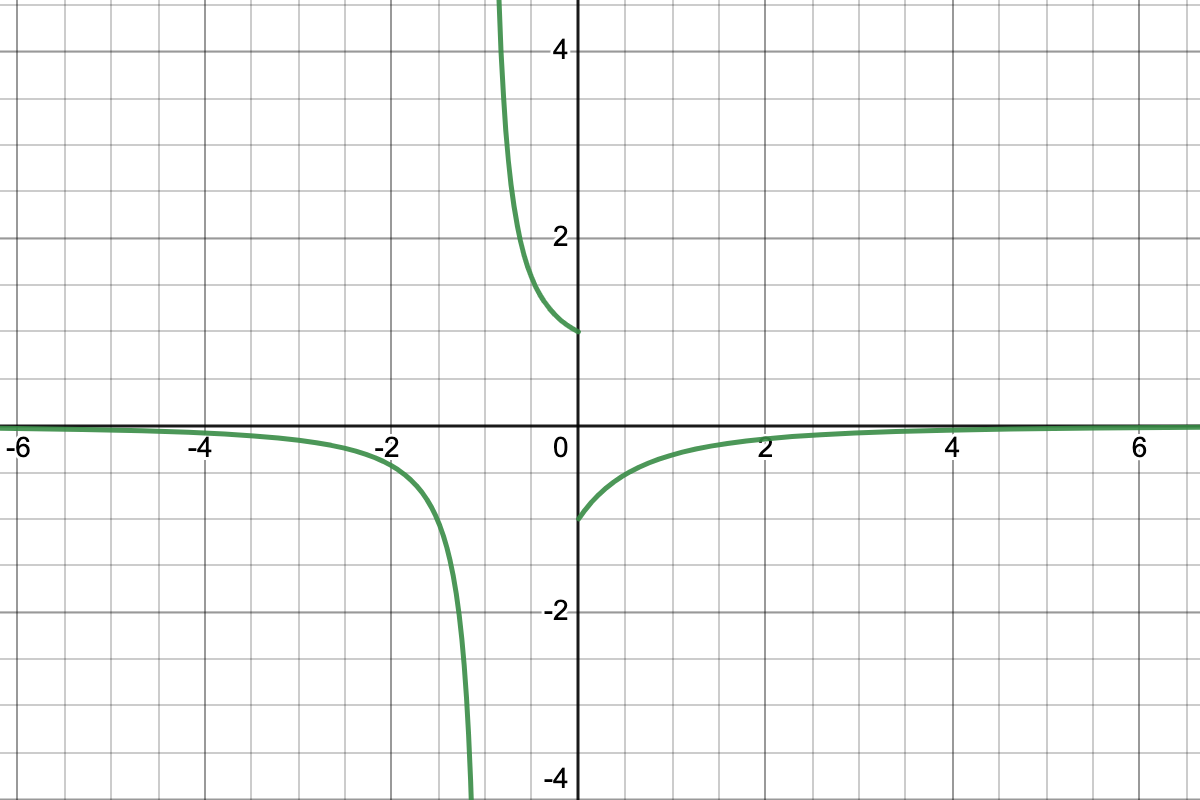
\includegraphics[width=0.6\textwidth]{src/disegno1.png}
        \caption{}
        \label{fig:1.1}
    \end{figure}
    \item Determinare $\dom F$
    Osserviamo che $0\in \dom f$, in quanto $F(0)=\int_0^0f(s)ds$
    \begin{itemize}
        \item se $x \in ]0,+\infty[$
        \[f(s)\underset{s\to0^+}{\longrightarrow}-1~~~f(s)\underset{s\to0^-}{\longrightarrow}1\]
        e la funzione è limitata in $]0,+\infty[$, per cui $f\in \mathcal{R}(]0,+\infty[)$
        \item se $x\in]-1,0[$\\
        $f(s)$ è continua in $]-1,0[$ e $f(s)\underset{s\to0^-}{\longrightarrow}1$, per cui l'integrale converge $\forall x\in [a,0[$ con $a\in ]-1,0[$.
        Dobbiamo controllare se converge in $-1$
        \[\int_0^{-1}f(s)ds=\int_0^{-1}\frac{e^s-1}{s(s+1)}ds\]
        per $s\to-1$ si ha 
        \[\frac{e^s-1}{s(s+1)}\sim \frac{\frac{1}{e}-1}{-1(s+1)}=\left( 1-\frac{1}{e} \right)\left( \frac{1}{s+1} \right)\]
        quindi l'integrale diverge negativamente per il criterio del confronto asintitico, da cui
        \[]-\infty,-1]\nsubseteq\dom F\]
    \end{itemize}
    Abbiamo quindi che $\dom F=]-1;+\infty[$
    \item Determinare $G_F$\\
    Per definizione di funzione integrale sappiamo che $F(0)=0$, inoltre per il teorema fondamentale del calcolo
    \[F'(x)=f(x)\begin{cases}
        <0&\se -1<x<0\\
        >0&\se x>0
    \end{cases}\]
    \[F''(x)=f'(x)\begin{cases}
        <0&\se -1<x<0\\
        >0&\se x>0
    \end{cases}\]
    Per il corollario di Lagrange
    \[F'_-(0)=\lim_{x\to0^-}f(x)=1\neq -1=\lim_{x\to0^+}f(x)=F'_+(0)\]
    per cui in $x=0$ la funzione presenta un punto angoloso.
    Siamo quindi in grado di determinare il grafico di $F$ (Figura \ref(fig:1.2)):
    \begin{figure}[ht]
        \centering
        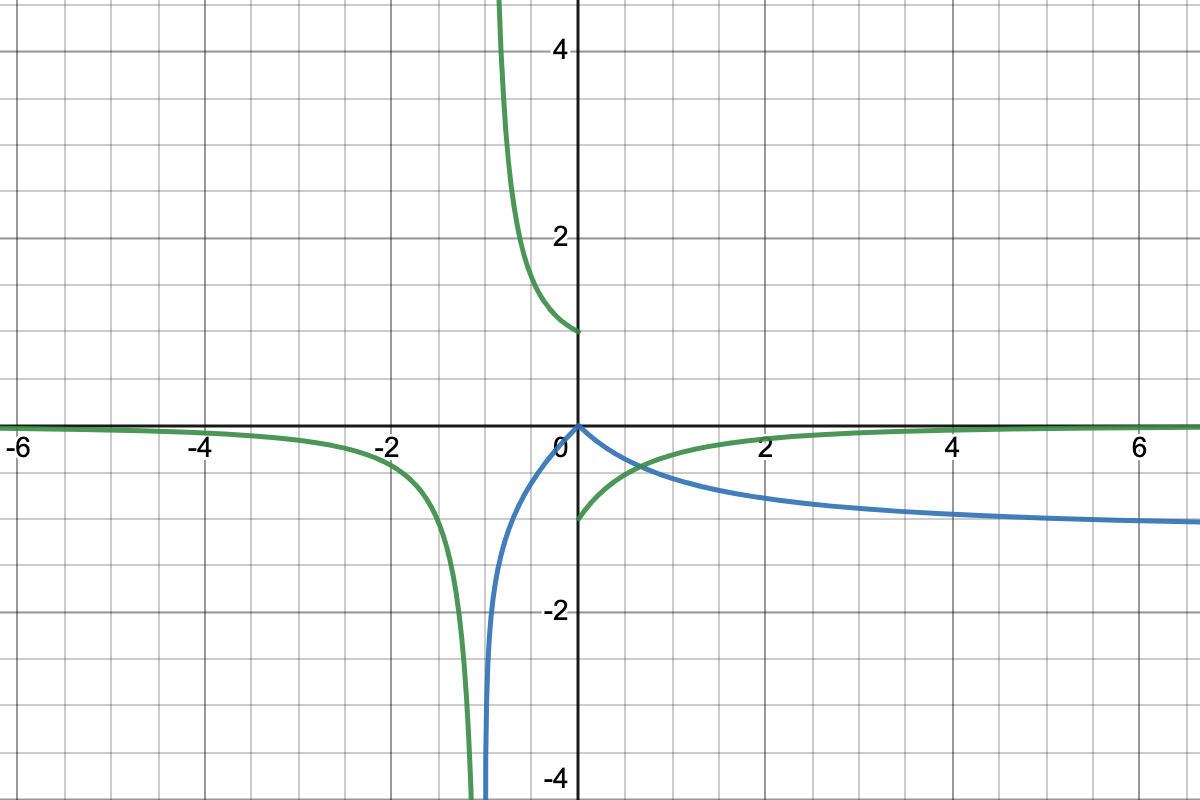
\includegraphics[width=0.6\textwidth]{src/disegno2.png}
        \caption{}
        \label{fig:1.2}
    \end{figure}
\end{enumerate}

%%%%%%%%%%%%%%%%%%%%%%%%%%%%%%%%%%%%%%%%%%%%%%%%%%%%%
Ricordiamo la definizione di convessità
\begin{shaded}
    \begin{definition}[Convessità]
        Sia $f:[a,b]\to\R$, $f$ si dice convessa se e solo se
        \[\forall x_1,x_2\in [a,b]~~~~~f(x)\leq f(x_1)+\frac{f(x_2)-f(x_1)}{x_2-x_1}\]
    \end{definition}
\end{shaded}
\item Dimostrare che una funzione $f:[a,b]\to\R$ è convessa se e solo se vale la seguente disuguaglianza
\[f(\lambda x_1+(1-\lambda)x_2)\leq \lambda f(x_1)+(1-\lambda)f(x_2)~~~\forall \lambda \in [0,1], \forall x_1,x_2\in [a,b]\]
\item[\textit{\large Soluzione~}]~
\begin{proof}~
    \begin{itemize}
        \item \say{$\Rightarrow$}
        Prendo $x \in [x_1,x_2]$
        \item \say{$\Leftarrow$}
    \end{itemize}
\end{proof}
\end{enumerate}
\[\christmaswedge\]
\end{document}
